\documentclass[11pt,english,letterpaper,oneside]{article}
\usepackage{amsmath,amssymb,amsfonts,amsthm,enumerate,enumitem}
\usepackage[top=3cm,bottom=3cm,left=2.5cm,right=2.5cm]{geometry}
\usepackage{graphicx,microtype}
\usepackage{textcomp}
\usepackage[T1]{fontenc}
\DisableLigatures[f]{encoding=T1}
\usepackage[skip=2pt]{caption}
\usepackage{hyperref,lineno}
\linenumbers
\usepackage{setspace,array,float}
\usepackage{bm,upgreek}
\usepackage[compact]{titlesec}
\usepackage[none]{hyphenat}
\setlength{\parskip}{0cm}
\usepackage{natbib}
\setcitestyle{citesep={;},aysep={}}
\usepackage{babel}
\usepackage{datetime}
\pagestyle{plain}
\frenchspacing
\doublespacing
\usepackage{sectsty}
\usepackage[table]{xcolor}
\allsectionsfont{\bfseries}

\makeatletter
\g@addto@macro\normalsize{%
  \setlength\belowdisplayskip{15pt}
  \setlength\belowdisplayshortskip{10pt}
}
\makeatother

%%%%%%%%%%%%%%%%%%%%%%%%%%%%%%%%%%%%%%%%%%%%%%%%%

\begin{document}

\newcommand{\tmat}{$\bm{T}$}
\newcommand{\rmat}{$\bm{R}$}
\newcommand{\etal}{\textit{et al}.}
\newdateformat{mydate}{\THEDAY{} \monthname[\THEMONTH], \THEYEAR}

\hfill Version dated: \mydate\today
\vspace{0.25in}

\begin{center}

{\LARGE  \bfseries Accounting for genotype uncertainty in the estimation of allele frequencies in autopolyploids}
\vspace{0.45in}

Paul D. Blischak$^{1,\dagger}$, Laura S. Kubatko$^{1,2}$ and Andrea D. Wolfe$^1$
\vspace{0.45in}


\textit{$^1$Department of Evolution, Ecology and Organismal Biology, The Ohio State University,}

\textit{318 W. 12th Avenue, Columbus, OH 43210, USA.}
\bigskip
\bigskip

\textit{$^2$Department of Statistics, The Ohio State University,}

\textit{1958 Neil Avenue, Columbus, OH 43210, USA.}


\end{center}
\vspace{0.45in}


\noindent $^\dagger$\textbf{Corresponding author}: Paul Blischak, The Ohio State University, Dept. of Evolution, Ecology and Organismal Biology, 318 W. 12th Avenue, Columbus, OH 43210. E-mail: blischak.4@osu.edu.

\vspace{0.45in}

\noindent \textbf{Running title}: Genotype uncertainty in autopolyploids

\vspace{.45in}

%%%%%%%%%%%%%%%%%%%%
\section*{Abstract}                      %%
%%%%%%%%%%%%%%%%%%%%

Despite the ever increasing opportunity to collect large-scale datasets for population genomic analyses, the use of high throughput sequencing to study populations of polyploids has seen little application. This is due in large part to problems associated with determining allele copy number in the genotypes of polyploid individuals (allelic dosage uncertainty--ADU), which complicates the calculation of important quantities such as allele frequencies. This well-known problem has hindered population genetic studies in polyploids for decades, though several tools exist for analyzing genetic data from polyploids by dealing with particular issues of ADU. Additional complications arise because of the mixed inheritance patterns and variable reproductive modes that are characteristic of many polyploid taxa, making the development of population genetic models for polyploids especially difficult. Here we describe a statistical model to estimate biallelic SNP frequencies in a population of autopolyploids using high throughput sequencing data in the form of read counts. Uncertainty in the number of copies of an allele in an individual's genotype is accounted for by treating genotypes as a latent variable in a hierarchical Bayesian model. In this way, we bridge the gap from data collection (using techniques such as restriction-site associated DNA sequencing) to allele frequency estimation in a unified inferential framework by summing over genotype uncertainty. Simulated datasets were generated under various conditions for both tetraploid and hexaploid populations to evaluate the model's performance and to help guide the collection of empirical data. We also discuss potential extensions to generalize our model and its application to polyploids.
\vspace{0.25in}

\noindent (\textbf{Keywords}: allelic dosage uncertainty, allele frequencies, hierarchical Bayesian modeling, polyploidy, population genomics)
\vspace{0.25in}

%%%%%%%%%%%%%%%%%%%
\section*{Introduction}            %%
%%%%%%%%%%%%%%%%%%%

Biologists have long been fascinated by the occurrence of whole genome duplication (WGD) in natural populations and have recognized its role in the generation of biodiversity \citep{ClausKeckHies1940,StebbinsVariationEvolution,GrantPlantSpeciation,otto2000polyploidy}. Though WGD is thought to have occurred at some point in nearly every branch of the Tree of Life (plants, animals and fungi), it is a particularly common phenomenon in plants and is regarded by many to be an important factor in plant diversification \citep{wood2009polyploid,soltisd2009diversification,scarpino2014polyploid}. The role of polyploidy in plant evolution was originally considered by some to be a ``dead-end'' \citep{StebbinsVariationEvolution,wagner1970noise,soltisd2014stebbins} but, since its first discovery in the early twentieth century, polyploidy has been continually studied in nearly all areas of botany \citep{winge1917polyploidy,Winkler1916polyploidy,ClausKeckHies1945polyploidy,GrantPlantSpeciation,StebbinsVariationEvolution,soltisD2003polyploid,soltisd2010polyploidUnknowns,soltai2009roleOfHybridization,ramsey2014polEcoProcRoySoc}. Though fewer examples of WGD are currently known for animal systems, groups such as amphibians, fish, and reptiles all exhibit polyploidy \citep{allendorf1984tetraploidFish,gregory2005polyploidyAnimals}. Ancient genome duplications are also thought to have played an important role in the evolution of both plants and animals, occurring in the lineages preceeding the seed plants, angiosperms and vertebrates \citep{ohno1970geneDuplication,otto2000polyploidy,furlong2001animalOctoploid,jiao2011ancientWGD}. These ancient WGD events during the early history of seed plants and angiosperms have been followed by several more WGDs in all major plant groups \citep{cui2006genomeDuplication,scarpino2014polyploid,canon2014polyploidyLegumes}. Recent experimental evidence has also demonstrated increased survivorship and adaptability to foreign environments of polyploid taxa when compared with their lower ploidy relatives \citep{ramsey2011polyploidEcology,Selmecki2015yeastAdaptation}.
\medskip

Polyploids are generally divided into two types based on how they are formed: auto- and allopolyploids. Autopolyploids form when a WGD event occurs within a single evolutionary lineage and typically have polysomic inheritance. Allopolyploids are formed by hybridization between two separately evolving lineages followed by WGD and are thought to have mostly disomic inheritance. Multivalent chromosome pairing during meiosis can occur in allopolyploids, however, resulting in mixed inheritance patterns across loci in the genome [segmental allopolyploids] \citep{StebbinsVariationEvolution}. Autopolyploids can also undergo double reduction, a product of multivalent chromosome pairing wherein segments from sister chromatids move together during meiosis---resulting in allelic inheritance that breaks away from a strict pattern of polysomy \citep{haldane1930autopolyploids}. It was also thought that autopolyploids were far less common than allopolyploids, but recent studies have concluded that autopolyploidy occurs more frequently than originally proposed \citep{soltis2007autopolyploidy,parisod2010autopolyploidy}.
\medskip

The theoretical treatment of population genetic models in polyploids has it origins in the Modern Synthesis with  Fisher, Haldane and Wright each contributing to the development of some of the earliest mathematical models for understanding the genetic patterns of inheritance in polyploids. Among the first of these works was Haldane's 1930 paper on autopolyploid inheritance in $2k$-ploid ($k=2,3,\dots$) organisms. Influenced in part by the works of Hermann J. Muller in tetraploid species of \textit{Primula} (\citeyear{muller1914primula}) and W. J. C. Lawrence in octoploid species of \textit{Dahlia} (\citeyear{lawrence1929dahlia}), Haldane generalized the combinatorial formulas for determining the frequencies of the different possible gametes formed from all genotype combinations for a $2k$-ploid. He also considered additional factors influencing gamete frequencies such as double reduction and the effects of partial selfing \citep{haldane1930autopolyploids}. Fisher's interest in polyploidy stemmed largely from observations made in the plant genus \textit{Lythrum}, which exhibited conspicuous patterns of trimorphic heterostyly \citep{fisher1941lythrum}. Empirical works by Nora Barlow (\citeyear{barlow1913heterostylism}, \citeyear{barlow1923trimorphic}), as well as initial investigations into the inheritance patterns of the three style types (Short, Mid, Long) by E. M. East (\citeyear{east1927lythrum}) formed the basis for Fisher's formulation of a model for the inheritance patterns of the Mid length style form in \textit{Lythrum salicaria} \citep{fisher1941lythrum}. He later added to this work by considering double reduction in the inheritance of the Mid length style and complemented his theoretical work through a collaboration with Kenneth Mather to complete crossing experiments \citep{fisher1943doublereduction,fisher1943mather}. Wright's contributions were concerned with the calculation of the distribution of allele frequencies in a $2k$-ploid and were largely an extension of his classic 1931 paper, \textit{Evolution in Mendelian populations}, and a previously published manuscript describing similar processes in diploids \citep{wright1931mendelianPops,wright1937geneFreqs,wright1938polyploid}. Wright was among the first to consider mutation, migration, selection and inbreeding in his formulation of the distribution of gene frequencies, which helped to establish future ideas about modeling allelic diffusion in a population. For example, it was noted by Kimura (\citeyear{kimura1964diffusion}) that much of the work on diffusion equations in population genetics could be applied to polyploids in a manner similar to Wright's derivation of the allele frequency distribution in polyploids.
\medskip

The foundation laid down by these early papers has led to the continuing development of population genetic models for polyploids, including models for understanding the rate of loss of genetic diversity and extensions of the coalescent in autotetraploids, as well as modifications of the multispecies coalescent for the inference of species networks containing allotetraploids \citep{moody1993autopolyploids,arnold2012autotetraploidCoal,jones2013allopolyploid}. Much of this progress was described in a review by Dufresne \etal{} (\citeyear{dufresne2014polyPopGen}), who outlined the current state of population genetics in polyploids regarding both molecular techniques and statistical models. Not surprisingly, one of the most promising developments for the future of population genetics in polyploids is the advancement of sequencing technologies. A particularly common method of gathering large datasets for genome scale inferences is restriction-site associated DNA sequencing [RADseq] \citep{miller2007gbs,baird2008radTags,puritz2014demystifyingRAD}. However, despite its popularity for population genetic inferences at the diploid level, there are much fewer examples of RADseq experiments conducted on polyploid taxa \citep[but see][]{ogden2013sturgeonRADseq,wang2013birchRADseq,logan-young2015polyploidSNP}. Among the primary reasons for the dearth in applying RADseq to polyploids is the issue of allelic dosage uncertainty (ADU), or the inability to fully determine the genotype of a polyploid organism when it is partially heterozygous. This is the same problem that has been encountered by other codominant markers such as microsatellites, which are commonly used for population genetic analyses in polyploids. One way of dealing with allelic dosage that has been used for multi-allelic microsatellite markers has been to code alleles as either present or absent based on their electropherogram readings and to analyze the resulting dominant data using a program such as \textsc{polysat} \citep{clark2007polysat,dufresne2014polyPopGen}. Attempts to infer the genotype of polyploid microsatellite loci have also been successfully completed in some cases by using the relative dosage of the alleles in the genotypes \citep{esselink2004polyploidSSR}. The situation would be similar for biallelic (allele A or B) SNP data collected using RADseq, where a partially heterozygous polyploid will have high throughput sequencing reads containing both the A and the B allele. For a tetraploid, the possible genotypes would then be AAAB, AABB and ABBB. For a hexaploid they are AAAAAB, AAAABB, AAABBB, AABBBB and ABBBBB. In general, the number of possible genotypes for a biallelic locus of a partially heterozygous K-ploid ($\text{K}=3,4,5,\ldots$) is $\text{K}-1$. A possible solution to this problem for SNPs would be to try to use existing genotype callers and to rely on the relative dosage of sequencing reads containing the two alleles (similar to what was done for microsatellites). However, this could lead to erroneous inferences when genotypes are simply fixed at point estimates based on read proportions without considering estimation error. Furthermore, when sequencing coverage is low, the number of genotypes that will appear to be equally probable increases with ploidy, making it difficult to distinguish among the possible partially heterozygous genotypes.
\medskip

In this paper we describe a model that aims to address the problems associated with ADU by treating genotypes as a latent variable in a hierarchical Bayesian model and using read counts as data (Figure \ref{fig:model-graph}). In this way, we preserve the uncertainty that is inherent in the genotypes of partially heterozygous polyploids by inferring a probability distribution across all possible values of the genotype, rather than treating the genotypes as being directly observed. Our model assumes that the ploidy level of the population is known and that the genotypes of individuals in the population are drawn from a single underlying allele frequency for each locus. These assumptions imply that alleles in the population are undergoing polysomic inheritance without double reduction, which most closely adheres to the inheritance patterns of an autopolyploid. We acknowledge that the model in its current form is an oversimplification of biological reality and realize that it does not apply to a large portion of polyploid taxa. Nevertheless, we believe that accounting for ADU by modeling genotype uncertainty has the potential to be applied more broadly via modifications of the probability model used for the inheritance of alleles, which could lead to more generalized population genetic models for polyploids (see the \textbf{Extensibility} section of the \textbf{Discussion}). 
\medskip

%%%%%%%%%%%%%%%%%%%%%%%%
\section*{Materials and Methods}        %%
%%%%%%%%%%%%%%%%%%%%%%%%

\noindent Our goal is to estimate the frequency of a reference allele for each locus sampled from a population of known ploidy ($\psi$), where the reference allele can be chosen arbitrarily between the two alleles at a given biallelic SNP. To do this we extend the population genomic models of \cite{buerkle2013popModels}, which employ a Bayesian framework to model high throughput sequencing reads ($\bm{T},\bm{R}$), genotypes ($\bm{G}$) and allele frequencies ($\bm{p}$), to the case of arbitrary ploidy. The idea behind the model is to view the sequencing reads gathered for an individual as a random sample from the unobserved genotype at each locus. Genotypes can then be treated as a parameter in a probability model that governs how likely it is that we see a particular number of sequencing reads carrying the reference allele. Similarly, we can treat genotypes as a random sample from the underlying allele frequency in the population (assuming Hardy-Weinberg equilibrium). For our model, a genotype is simply a count of the number of reference alleles at a locus which can range from 0 (a homozygote with no reference alleles in the genotype) to $\psi$ (a homozygote with only reference alleles in the genotype). All whole number in between 0 and $\psi$ represent partially heterozygous genotypes. This hierarchical setup addresses the problems associated with ADU by treating genotypes as a latent variable that can be integrated out using Markov chain Monte Carlo (MCMC).

\medskip
\subsection*{Model setup}
\medskip

Here we consider a sample of $N$ individuals from a single population of ploidy level $\psi$ sequenced at $L$ unlinked SNPs. The data for the model consist of two matrices containing counts of high throughput sequencing reads mapping to each locus for each individual: \rmat{} and \tmat. The $N \times L$ matrix \tmat{} contains the total number of reads sampled at each locus for each individual. Similarly, \rmat{} is an $N \times L$ matrix containing the number of sampled reads with the reference allele at each locus for each individual. Assuming conditional independence of the sequencing reads given genotypes, the probability distribution for sequencing reads can be factored as

\begin{equation}\label{factored_lik}
P(\bm{R}|\bm{T},\bm{G}, \epsilon) = \displaystyle\prod_{\ell=1}^L\displaystyle\prod_{i=1}^N P(r_{i \ell}|t_{i \ell},g_{i \ell}, \epsilon)\,.
\end{equation}

\noindent Then for an individual, $i$, at locus $\ell$, we model the number of sequencing reads containing the reference allele ($r_{i\ell}$) as a Binomial random variable conditional on the total number of sequencing reads ($t_{i\ell} $), the underlying genotype ($g_{i\ell}$) and a constant level of sequencing error ($\epsilon$)

\begin{equation}\label{likelihood}
P(r_{i \ell}|t_{i\ell}, g_{i \ell},\epsilon) = \binom{t_{i \ell}}{r_{i \ell}}
	\begin{cases}
	\epsilon^{r_{i \ell}}(1-\epsilon)^{t_{i \ell}-r_{i \ell}} & \text{if  } g_{i \ell} = 0, \\[0.05in]
	\left(\frac{g_{i \ell}}{\psi}\right)^{r_{i \ell}}\left(1-\frac{g_{i \ell}}{\psi}\right)^{t_{i \ell}-r_{i \ell}} & \text{if  } g_{i \ell} = 1,\ldots,\psi-1, \\[0.05in]
	(1-\epsilon)^{r_{i \ell}}\epsilon^{t_{i \ell}-r_{i \ell}} & \text{if  } g_{i \ell} = \psi\,.
	\end{cases}
\end{equation}


\noindent Since the $r_{i \ell}$'s are the data that we observe, the product of $P(r_{i \ell}|t_{i\ell}, g_{i \ell},\epsilon)$ across loci and individuals will form the likelihood in the model. An important consideration here is that when $g_{i \ell}$ is equal to 0 or $\psi$ (i.e., when the genotype is homozygous) but the sequence data collected for the individual contains both alleles, the likelihood will be 0. To correct for this, we include error ($\epsilon$) into the model. The intuition behind including error is that reads sampled from a locus that is truly homozygous can still contain more than one allele due to sequencing errors, giving the false impression that the individual may be a partial heterozygote. If we assume that the probability of a sequencing error is smaller than the probability of being truly heterozygous (i.e., containing at least one reference allele in the genotype), then the probability model we use for reference reads should be able to distinguish between homozygotes with reads containing sequencing errors and partial heterozygotes. When we do this, the probability distribution for $r_{i\ell}$ given $g_{i\ell}$ and $\epsilon$ is split into $\psi+1$ cases as above in Eq. \ref{likelihood}.
\medskip

The next level in the hierarchy is the conditional prior for genotypes. We assume that the genotypes of the sampled individuals are conditionally independent given the allele frequencies ($\bm{p}$), which is equivalent to taking a random sample from a population in Hardy-Weinberg equilibrium. Factoring the distribution for genotypes and taking the product across loci and individuals gives us the joint probability distribution of genotypes given the ploidy level of the population and the allele frequencies at each locus ($p_{\ell}$):

\begin{equation}\label{condl_prior}
P(\bm{G}|\psi, \bm{p}) = \displaystyle\prod_{\ell=1}^L\displaystyle\prod_{i=1}^N P(g_{i \ell}|\psi, p_{\ell})\,.
\end{equation}

\noindent We model each $g_{i \ell}$ as a Binomial random variable conditional on the ploidy level of the population and the frequency of the reference allele for locus $\ell$:

\begin{equation*}
P(g_{i \ell}|\psi,p_{\ell}) = \binom{\psi}{g_{i \ell}}\,p_{\ell}^{g_{i \ell}}(1-p_{\ell})^{\psi-g_{i \ell}}\,.
\end{equation*}

The final level of the model is the prior distribution on allele frequencies. Assuming \textit{a priori} independence across loci, we use a Beta distribution with parameters $\alpha$ and $\beta$ both equal to $1$ as our prior distribution for each locus. A Beta(1,1) is equivalent to a Uniform distribution over the interval $[0,1]$, making our choice of prior uninformative. The joint posterior distribution of allele frequencies and genotypes is then equal to the product across all loci and all individuals of the likelihood, the conditional prior on genotypes and the prior distribution on allele frequencies up to a constant of proportionality

\begin{align}\label{posterior}
P(\,\bm{p},\bm{G}|\bm{R},\epsilon) &\propto P(\bm{R}|\bm{T},\bm{G}, \epsilon)P(\bm{G}|\psi,\bm{p})P(\bm{p}) \nonumber \\[0.05in]
&= \displaystyle\prod_{\ell=1}^L\displaystyle\prod_{i=1}^N P(r_{i \ell}|t_{i\ell}, g_{i \ell},\epsilon)P(g_{i \ell}|\psi, p_{\ell})P(p_{\ell})\,.
\end{align}

\noindent The marginal posterior distribution for allele frequencies can be obtained by summing over genotypes

\begin{equation}\label{marg_post_p}
P(\,\bm{p}|\bm{R},\epsilon) \propto \displaystyle\sum_{\bm{G}} P(\,\bm{p},\bm{G}|\bm{R},\epsilon)\,.
\end{equation}

\noindent It would also be possible to examine the marginal posterior distribution of genotypes but here we will only focus on allele frequencies (see \textbf{Discussion} for potential applications of the marginal distribution of genotypes).

\medskip
\subsection*{Full conditionals and MCMC using Gibbs sampling}
\medskip

\noindent We estimate the joint posterior distribution for allele frequencies and genotypes in Eq. \ref{posterior} using MCMC. This is done using Gibbs sampling of the states $(\,\bm{p},\bm{G})$ in a Markov chain by alternating samples from the full conditional distributions of $\bm{p}$ and $\bm{G}$. Given the setup for our model using Binomial and Beta distributions (which form a conjugate family), analytical solutions for these distributions can be readily acquired \citep{gelman2014bayesian}. The full conditional distribution for allele frequencies is Beta distributed and is given by Eq. \ref{p-full} below:

\begin{equation}\label{p-full}
p_{\ell}\,|\,g_{i \ell},r_{i \ell},\epsilon \: \sim \: \text{Beta}\left(\alpha= \sum_{i=1}^N g_{i \ell} +1,\; \beta = \sum_{i=1}^N (\psi-g_{i \ell})+1\right),\quad \text{for } \ell = 1,\ldots,L.
\end{equation}

\noindent This full conditional distribution for $p_{\ell}$ has a natural interpretation as it is roughly centered at the proportion of sampled alleles carrying the reference allele divided by the total number of alleles sampled given the current state of $\bm{G}$ in the Markov chain. The ``$+1$'' comes from the prior distribution and won't have a strong influence on the posterior when the sample size is large.
\medskip

The full conditional distribution for genotypes is split into $\psi+1$ cases (similar to the conditional prior), making it a discrete categorical distribution over the possible values for the genotypes $(0,\ldots,\psi)$. Using $k$ as a generic index, the distribution for individual $i$ at locus $\ell$ is

\begin{equation}\label{G-full}
P(g_{i \ell}|g_{(\text{-}i) \ell},p_{\ell},r_{i \ell},\epsilon) = \frac{1}{\mathcal{C}_{i \ell}} \;
	\begin{cases}
	\epsilon^{r_{i \ell}}(1-\epsilon)^{t_{i \ell}-r_{i \ell}}(1-p_{\ell})^\psi & \text{for  } k = 0, \\[0.05in]
	\left(\frac{k}{\psi}\right)^{r_{i \ell}}\left(1-\frac{k}{\psi}\right)^{t_{i \ell}-r_{i \ell}}\displaystyle\binom{\psi}{k}p_{\ell}^{k}\,(1-p_{\ell})^{\psi-k} & \text{for  } k = 1,\ldots,\psi-1, \\[0.05in]
	(1-\epsilon)^{r_{i \ell}}\epsilon^{t_{i \ell}-r_{i \ell}}p_{\ell}^\psi & \text{for  } k = \psi\,,
	\end{cases} 
\end{equation}

\noindent where $g_{(\text{-}i) \ell}$ is the value of the genotypes for all sampled individuals excluding individual $i$ and $\mathcal{C}_{i \ell}$ is a normalizing constant equal to the sum of all of the terms:

\begin{equation*}
\mathcal{C}_{i \ell} = \epsilon^{r_{i \ell}}(1-\epsilon)^{t_{i \ell}-r_{i \ell}}(1-p_{\ell})^\psi + (1-\epsilon)^{r_{i \ell}}\epsilon^{t_{i \ell}-r_{i \ell}}p_{\ell}^\psi + \sum_{k=1}^{\psi-1}\left(\left(\frac{k}{\psi}\right)^{r_{i \ell}}\left(1-\frac{k}{\psi}\right)^{t_{i \ell}-r_{i \ell}}\binom{\psi}{k}\,p_{\ell}^k(1-p_{\ell})^{\psi-k}\right).
\end{equation*}

\noindent The full conditional distribution for genotypes can be seen as the product of two quantities: (1) the probability of each of the possible genotypes based on the observed  reference reads and (2) the probability of drawing each genotype value based on the current value for the frequency of the reference allele for locus $\ell$ in the population. 

We begin our Gibbs sampling algorithm in a random position in parameter space through the use of uniform probability distributions. The genotype matrix is initialized with random draws from a Discrete Uniform distribution from $0$ to $\psi$ and the initial allele frequencies are drawn from a Uniform distribution on the interval [0,1]. 

\medskip
\subsection*{Simulation study}
\medskip

Simulations were performed to assess error rates in allele frequency estimation for tetraploid and hexaploid populations ($\psi$ = 4 and 6, respectively). Data were generated under the model by sampling genotypes from a binomial distribution conditional on a fixed, known allele frequency $(\,p_{\ell} = 0.01, 0.05, 0.1, 0.2, 0.4)$. Total read counts were simulated for a single locus using a Poisson distribution with mean coverage equal to 5, 10, 20, 50 or 100 reads per individual. We then sampled the number of sequencing reads containing the reference allele from a binomial distribution conditional on the number of total reads, the genotype and sequencing error (Eq. \ref{likelihood}; $\epsilon$ fixed to 0.01). Finally, we varied the number of individuals sampled per population $(N = 5, 10, 20, 30)$ and ran all possible combinations of the simulation settings. Each combination of sequencing coverage, individuals sampled and allele frequency was analyzed using 100 replicates for both tetraploid and hexaploid populations for a total of  20,000 simulation runs. MCMC analyses using Gibbs sampling were run for 100,000 generations with parameter values stored every 100 samples. The first 25\% of the posterior was discarded as burn-in, resulting in 750 posterior samples for each replicate. Convergence on the stationary distribution, $P(\,\bm{p},\bm{G}|\bm{R},\epsilon)$, was assessed by examining trace plots for a subset of runs for each combination of settings and ensuring that the effective sample sizes (ESS) were greater than 200. Deviations from the known underlying allele frequency used to simulate each data set were assessed by calculating the posterior mean of each replicate, followed by subtracting the known value from the calculated means and then calculating their standard deviation.
\medskip

All simulations were performed using the R statistical package \citep{r2014} on the Oakley cluster at the Ohio Supercomputer Center (\url{https://osc.edu}). Figures were generated using the R packages \textsc{ggplot2} \citep{wickham2009ggplot2}, \textsc{reshape} \citep{wickham2011plyr} and \textsc{plyr} \citep{wickham2007reshape} with additional figure manipulation completed using Inkscape (\url{https://inkscape.org}). MCMC diagnostics were done using the \textsc{coda} package \citep{plummer2006coda}.
\medskip

%%%%%%%%%%%%%%%
\section*{Results}         %%
%%%%%%%%%%%%%%%

\subsection*{Gibbs sampler}
\medskip

Our Gibbs sampling algorithm was able to accurately estimate allele frequencies for a number of simulation settings while simultaneously allowing for genotype uncertainty. Convergence (ESS values > 200) was achieved for all simulation replicates and all trace plots examined also indicated that the Markov chain had reached stationarity (Figure S1). We have aggregated the scripts for our Gibbs sampler as a developmental R package---\textsc{polyfreqs}---which is available on GitHub (\url{https://github.com/pblischak/polyfreqs}). Though \textsc{polyfreqs} is written in R, it deals with the large datasets that are generated by high throughput sequencing platforms in two ways. First, it takes advantage of R's ability to incorporate C++ code via the \textsc{Rcpp} and \textsc{RcppArmadillo} packages, allowing for a faster implementation of our MCMC algorithm \citep{eddelbuettel2011rcpp,eddelbuettel2013rcppBook,eddelbuettel2014rcpparmadillo}. Second, since the model assumes independence among loci, \textsc{polyfreqs} can facilitate the process of parallelizing analyses by splitting the total read count and reference read count matrices into subsets of loci which can be analyzed at the same time on separate nodes of a computing cluster.

\medskip
\subsection*{Simulation study}
\medskip

Increasing the number of individuals sampled had the largest effect on the accuracy of allele frequency estimation (Figures \ref{fig:tetra-heatmaps} \& \ref{fig:hex-heatmaps}). Since allele frequencies are a population level parameter, it is not surprising that sampling more individuals from the population leads to better estimates. This appears to be the case even when sequencing coverage is quite low (5x, 10x), which corroborates the observations made by \cite{buerkle2013popModels}. Lower sequence coverage does effect the posterior distribution for allele frequencies even when the number of individuals sequenced is large however, by increasing the posterior standard deviation (Figure \ref{fig:coverage-sd}). An interesting pattern that emerged during the simulation study is the observation that the allele frequencies closer to 0.5 tend to have higher error rates.
\medskip

%%%%%%%%%%%%%%%%%
\section*{Discussion}         %%
%%%%%%%%%%%%%%%%%

The inference of population genetic parameters and the demographic history of non-model polyploid organisms has lagged behind that of diploids for decades. The difficulties associated with these inferences present themselves at two levels. The first of these is the widely known inability to determine the genotypes of polyploids due to ADU. Even though there have been theoretical developments in the description of models for polyploid taxa as early as the 1930s, a large portion of this population genetic theory relies on knowledge about individuals' genotypes \citep[e.g.,][]{haldane1930autopolyploids,wright1938polyploid}. The second complicating factor is the complexity of inheritance patterns and changes in mating systems that often accompany WGD events. Polyploid organisms can sometimes mate by both outcrossing or selfing, and can display mixed inheritance patterns at different loci in the genome \citep{dufresne2014polyPopGen}. If genotypes were known, then it might be easier to develop and test models for dealing with and inferring rates of selfing versus outcrossing, as well as understanding inheritance patterns across the genome. However, ADU only compounds the problems associated with these inferences, making the development and application of appropriate models far more difficult \citep[but see list of software in][]{dufresne2014polyPopGen}. The model we have presented here deals with the first of these two issues by not treating genotypes as observed quantities. Almost all other methods of genotype estimation for polyploids treat the genotype as the primary parameter of interest. Our model is different in that we still use the read counts generated by high throughput sequencing platforms as our observed data but instead integrate across genotype uncertainty when inferring other parameters, thus bypassing the problems caused by ADU.
\medskip

Despite our focus on bypassing ADU, an important consideration for the model we present here is that, because it approximates the joint posterior distribution of allele frequencies and genotypes, it would also be possible to use the marginal posterior distribution of genotypes to make inferences using existing methods. This could be done using the posterior mode as a maximum \textit{a posteriori} (MAP) estimate of the genotype for downstream analyses, followed by analyzing random samples from the posterior distribution of genotypes. The resulting set of estimates would not constitute a ``true'' posterior distribution of downstream parameters but would allow researchers to interpret their results based on the MAP estimate of the genotypes while still getting a sense for the amount of variation in their estimates. Using the posterior distribution of genotypes in this way could theoretically be applied to any type of polyploid, but is only really appropriate for autopolyploids due to the model of inheritance that is used. Other methods for estimating SNP genotypes from high throughput sequencing data include the program \textsc{SuperMASSA}, which models the relative intensity of the two alternative alleles using Normal densities \citep{serang2012supermassa}.
\medskip

A second important factor for using our model is that, although estimates of allele frequencies can be accurate when sequencing coverage is low and sample sizes are large, the distribution for genotypes is likely going to be quite diffuse. For analyses that treat genotypes as a nuisance parameter, this is not an issue since we can integrate across genotype uncertainty. However, if the genotype \textit{is} of primary interest, then the experimental design of the study will need to change to acquire higher coverage at each locus for more accurate genotype estimation. Therefore, the decision between sequencing more individuals with lower average coverage versus sequencing fewer individuals with higher average coverage depends primarily on whether the genotypes will be used or not.

\medskip
\subsection*{Model adequacy}
\medskip

As noted earlier, the probability model that we use for the inheritance of alleles is one of polysomy without double reduction. In some cases, this model may be inappropriate but it can still be informative to check for loci that do or do not follow the model that we assume. Below we describe a simple procedure for rejecting our model of inheritance on a per locus basis using comparisons with the posterior predictive distribution of sequencing reads. Model checking is an important part of making statistical inferences and can play a role in understanding when a model adequately describes the data being analyzed. In the case of our model, it can serve as a basis for understanding the inheritance patterns of the organism being studied by determining which loci adhere to a simple pattern of polysomic inheritance. 
\medskip

Given $M$ posterior samples for the allele frequencies at each locus, $\left\{p_{\ell}^{[1]},p_{\ell}^{[2]},\ldots,p_{\ell}^{[M]} \right\}$, we will simulate new values for the genotypes ($\tilde{g}_{i \ell}$) and reference read counts ($\tilde{r}_{i \ell}$) for all individuals and use the ratio of simulated reference read counts to observed total read counts $\left( \frac{\tilde{r}_{i \ell}}{t_{i \ell}} \right) $ as a summary statistic for comparing the observed read count ratios to the distribution of the predicted read count ratios. The use of the likelihood (or similar quantities) as a summary statistic has been a common practice in posterior predictive comparisons of nucleotide substitution models, and more recently for comparative phylogenetics \citep{ripplinger2010DNAmodels,reid2014poorfit,pennell2015adequacy}. We use the ratio of reference to total read counts here because it is the maximum likelihood estimate of the probability of success for a Binomial random variable and because it is a simple quantity to calculate. The use of other summary statistics, or a combination of multiple summary statistics, would also possible. The procedure for our posterior predictive model check is as follows:
\medskip

\begin{enumerate}
  \item For locus $\ell = 1,\ldots,L$:
  \begin{enumerate}[label={\arabic{enumi}.\arabic*.}]
    \item For posterior sample $m = 1,\ldots,M$:
    \begin{enumerate}[label={\arabic{enumi}.\arabic{enumi}.\arabic*.}]
      \item Simulate new genotype values $\left( \tilde{g}_{i \ell}^{[m]}\right)$ for all individuals ($i = 1,\ldots,N$) by drawing from a $\text{Binomial}\left( \psi,p_{\ell}^{[m]} \right)$.
      \item Simulate new reference read counts $\left( \tilde{r}_{i \ell}^{[m]} \right)$ from each new genotype for all individuals by drawing from Eq. \ref{likelihood}.
      \item Calculate the reference read ratio for the simulated data for sample $m$ and sum across individuals: $\mathcal{\tilde{S}}_{\ell}^{[m]} = \sum_{i=1}^{N} \left(\frac{\tilde{r}_{i \ell}^{[m]}}{t_{i \ell}} \right)$.
      \item Calculate the reference read ratio for the observed data and sum across individuals: $\mathcal{S}_{\ell} = \sum_{i=1}^{N} \left(\frac{r_{i \ell}}{t_{i \ell}} \right)$.
    \end{enumerate}
    \item Calculate the difference between the observed reference read ratio and the $M$ simulated reference read ratios: $\left\{ \mathcal{S}_{\ell}-\mathcal{\tilde{S}}_{\ell}^{[1]},\ldots,\mathcal{S}_{\ell}-\mathcal{\tilde{S}}_{\ell}^{[M]}\right\}$.
\end{enumerate}
\item Determine if the 95\% highest posterior density (HPD) interval of the distribution of re-centered reference read ratios contains 0.
\end{enumerate}
\medskip

When the distribution of the differences in ratios between the observed and simulated datasets does not contain 0 in the 95\% HPD interval, it provides evidence that the locus being examined does not follow a pattern of strict polysomic inheritance. A similar approach could be used on an individual basis by comparing the observed ratio of reference reads to the predicted ratios for each individual at each locus. We implement the per locus version of this posterior predictive model checking procedure in the \textsc{polyfreqs} package with the function \texttt{polyfreqs\_pps}.

\medskip
\subsection*{Extensibility}
\medskip

The modular nature of our hierarchical model allows for the addition and modification of nodes in the model graph (Figure \ref{fig:model-graph}). One of the simplest extensions to the model that can build directly off of the current setup would be to consider loci with more than two alleles. This can be done using Multinomial distributions for sequencing reads and genotypes and a Dirichlet prior on allele frequencies \citep[the Multinomial and Dirichlet distributions form a conjugate family;][]{gelman2014bayesian}. We could also model populations of mixed ploidy by using a vector of individually assigned ploidy levels instead of assuming a single value for the whole population $(\bm{\psi} = \{\psi_1,\ldots,\psi_N\})$. However, this would assume random mating among ploidy levels.
\medskip

The place where we believe our model could have the greatest impact is through modifications and extensions of the probability model used for the inheritance of alleles. These models have been difficult to apply in the past as a result of genotype uncertainty. However, using our model as a starting point, it could be possible to infer patterns of inheritance (polysomy, disomy, heterosomy) and other demographic parameters (e.g., effective population size, population differentiation) without requiring direct knowledge about the genotypes of the individuals in the population. For example, Haldane's (\citeyear{haldane1930autopolyploids}) model of genotype frequencies for autopolyploids that are partially selfing could be used to infer the prevalence of self-fertilization within a population. Similarly, Fisher's (\citeyear{fisher1943doublereduction}) model for double reduction in the inheritance of style lengths for \textit{Lythrum} could be generalized and used alone or together with a model for partial selfing to better understand how these processes affect the genetic diversity of a population. A more recent model described by \cite{stift2008polyploidInheritance} used microsatellites to infer the different inheritance patterns (disomic, tetrasomic, intermediate) for tetraploids in the genus \textit{Rorippa} (Brassicaceae) following crossing experiments. The reformulation of such a model for biallelic SNPs gathered using high throughput sequencing could provide a suitable framework for understanding inheritance patterns across the genome. An ideal model would be one that could help to understand inheritance patterns without the need conduct additional experiments. However, to our knowledge, such a model does not currently exist and may not even be possible to implement due to the complexity of possible inheritance patterns that might need to be considered without the addition of information from crosses.
\medskip

%%%%%%%%%%%%%%%%%
\section*{Conclusions}      %%
%%%%%%%%%%%%%%%%%

The recent emergence of models for genotype uncertainty in diploids has introduced a theoretical framework for dealing with the fact that genotypes are unobserved quantities \citep{gompert2012bgc,buerkle2013popModels}. Our extension of this theory to cases of higher ploidy (specifically to autopolyploids) progresses naturally from the original work but also serves to alleviate the deeper issue of ADU. The power and flexibility of these models as applied at the diploid level has the potential to be replicated for polyploid organisms with the addition of suitable models for allelic inheritance. The construction of hierarchical models containing suitable probability models for ADU, allelic inheritance and perhaps even additional levels for important parameters such as F statistics or the allele frequency spectrum also have the potential to provide key insights into the population genetics of polyploids \citep{gompert2011bamova,buerkle2013popModels}. Future work on such models will help to progress the study of polyploid taxa and could eventually lead to more generalized models for understanding the processes that have shaped their evolutionary histories.
\medskip

%%%%%%%%%%%%%%%%%%%%%%%
\section*{Acknowledgements}           %%
%%%%%%%%%%%%%%%%%%%%%%%

The authors would like to thank the Ohio Supercomputer Center for access to computing resources and Nick Skomrock for assistance with deriving the full conditional distributions of the model in the diploid case. We would also like to thank \textit{Associate Editor name} and \# anonymous reviewers for their comments on the manuscript. This work was partially funded through a grant from the National Science Foundation (DEB-1455399) to ADW and LSK.
\bigskip


%%%%%%%%%%%%%%%%%
% References                       %%
%%%%%%%%%%%%%%%%%

\singlespacing

\bibliographystyle{MolEcol}
\bibliography{references}

\doublespacing

%%%%%%%%%%%%%%%%%%%%%%%
\section*{Author Contributions}        %%
%%%%%%%%%%%%%%%%%%%%%%%

Conceived of the study: PDB, LSK and ADW. PDB derived the polyploid model, ran the simulations, coded the R package and wrote the initial draft of the manuscript. PDB, LSK and ADW reviewed all parts of the manuscript and all authors approved of the final version.
\medskip

%%%%%%%%%%%%%%%%%%%%%%
\section*{Data Accessibility}            %%
%%%%%%%%%%%%%%%%%%%%%%

Scripts for simulating the datasets, analyzing them using Gibbs sampling and producing the figures from the resulting output can all be found on GitHub (\url{https://github.com/pblischak/polyfreqs-ms-data}). We also provide an implementation of the Gibbs sampler for estimating allele frequencies in the developmental R package \textsc{polyfreqs} (\url{https://github.com/pblischak/polyfreqs}). See the package vignette or GitHub wiki for more details (\url{https://github.com/pblischak/polyfreqs/wiki}).

%%%%%%%%%%
% Tables          %%
%%%%%%%%%%

\begin{table}
\centering
\rowcolors{1}{white}{gray!25}
\caption{\textbf{Notation and symbols used in the description of the model for estimating allele frequencies in polyploids}. Vector and matrix forms of the variables are also provided when appropriate. }
\vspace{0.25in}
\bgroup
\def\arraystretch{1.45}
\begin{tabular}[l]{l | l}
\hline
\textbf{Symbol} & \textbf{Description}\\ \hline
$L$ & The number of loci. \\
$\ell$ & Index for loci ($\ell\; \in \{1,\ldots,L\}$). \\
$N$ & Total number of individuals sequenced. \\
$i$ & Index for individuals ($i\; \in \{1,\ldots,N\}$). \\
$\psi$ & The ploidy level of individuals in the population (e.g., tetraploid: $\psi$=4). \\
$p_{\ell}$ & Frequency of the reference allele at locus $\ell$. [$\bm{p}$] \\
$g_{i \ell}$ & The number of copies of the reference allele for individual $i$ at locus $\ell$. [$\bm{G}$] \\
$\tilde{g}_{i \ell}$ & Simulated genotype for posterior predictive model checking. \\
$t_{i \ell}$ & The total number of reads for individual $i$ at locus $\ell$. [$\bm{T}$] \\
$r_{i \ell}$ & The number of reads with the reference allele for individual $i$ at locus $\ell$. [$\bm{R}$] \\
$\tilde{r}_{i \ell}$ & Simulated reference read count for posterior predictive model checking. [$\tilde{\bm{R}}$] \\
$\epsilon$ & Sequencing error. \\
\hline
\end{tabular}
\egroup
\label{table1}
\vspace{0.25in}
\end{table}

%%%%%%%%%%%
% Figures           %%
%%%%%%%%%%%

% Put figures here...
\begin{figure}
\centering
\caption{\textbf{Graphical representation of a hierarchical Bayesian model for estimating allele frequencies}. The two levels (allelic dosage and inheritance) represent the probability models that are used for inference from one graph node to another. The model we present here focuses primarily on allelic dosage.}
\vspace{0.25in}
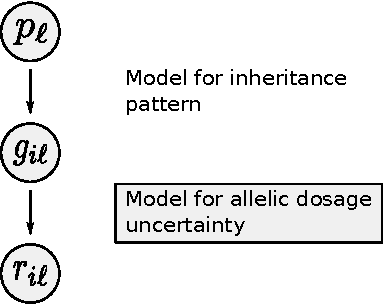
\includegraphics{fig/figure1-model-graph}
\label{fig:model-graph}
\end{figure}

\begin{figure}
\centering
\caption{\textbf{Heat maps of error rates for allele frequency estimation in tetraploids}. The x-axis shows the number of individuals (i5, i10, i20, i30) and the y-axis represents the sequencing coverage (c5, c10, c20, c50, c100) for each simulation. Note that the scales for each heat map are not the same, but the overall pattern of increased accuracy as the number of individuals and sequencing coverage increases for all allele frequencies.}
\vspace{0.25in}
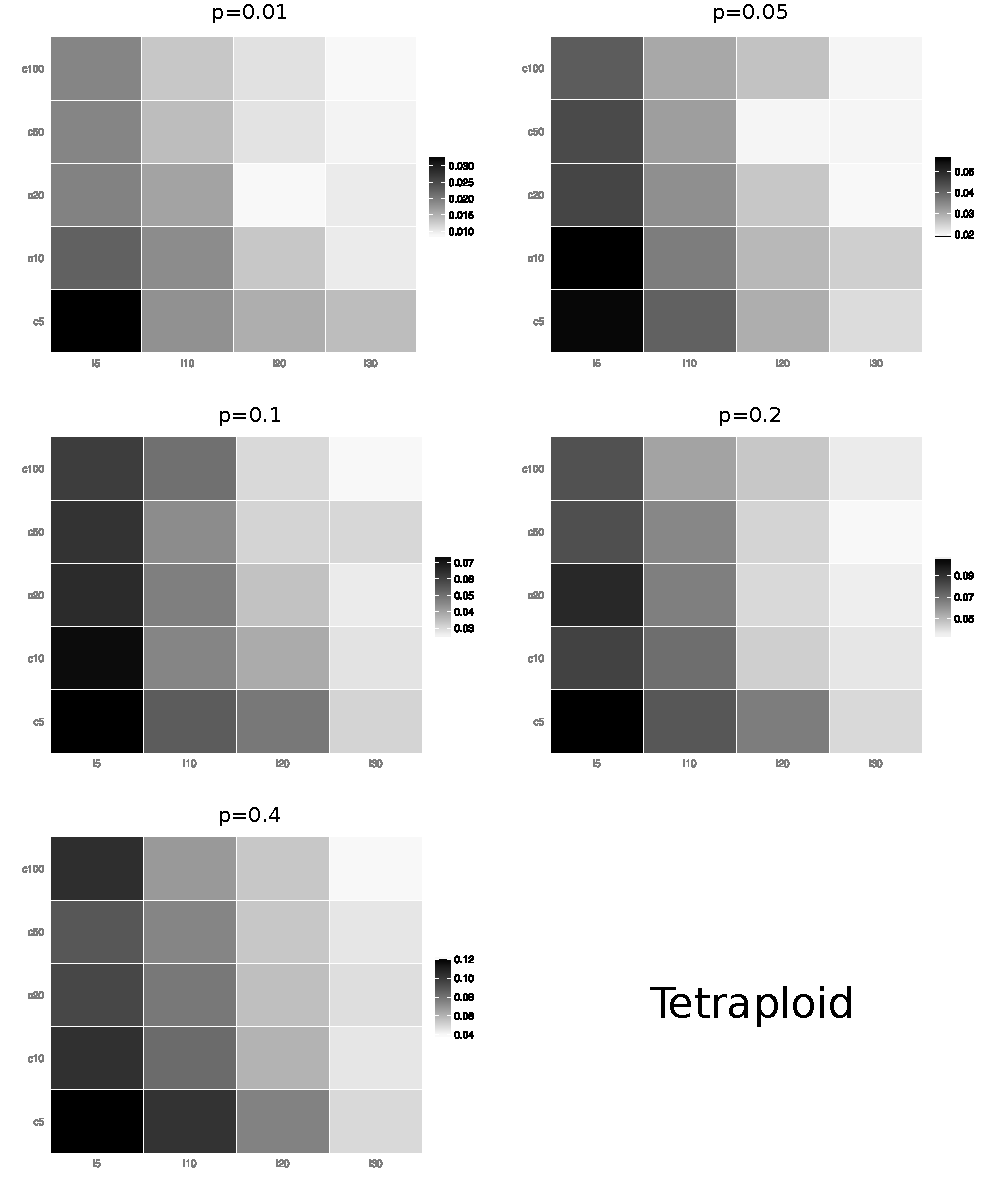
\includegraphics{fig/figure2-tetra-heatmaps}
\label{fig:tetra-heatmaps}
\end{figure}

\begin{figure}
\centering
\caption{\textbf{Heat maps of error rates for allele frequency estimation in hexaploids}. The x-axis shows the number of individuals (i5, i10, i20, i30) and the y-axis represents the sequencing coverage (c5, c10, c20, c50, c100) for each simulation. Note that the scales for each heat map  are not the same, but the overall pattern of increased accuracy as the number of individuals and sequencing coverage increases is the same for all allele frequencies.}
\vspace{0.25in}
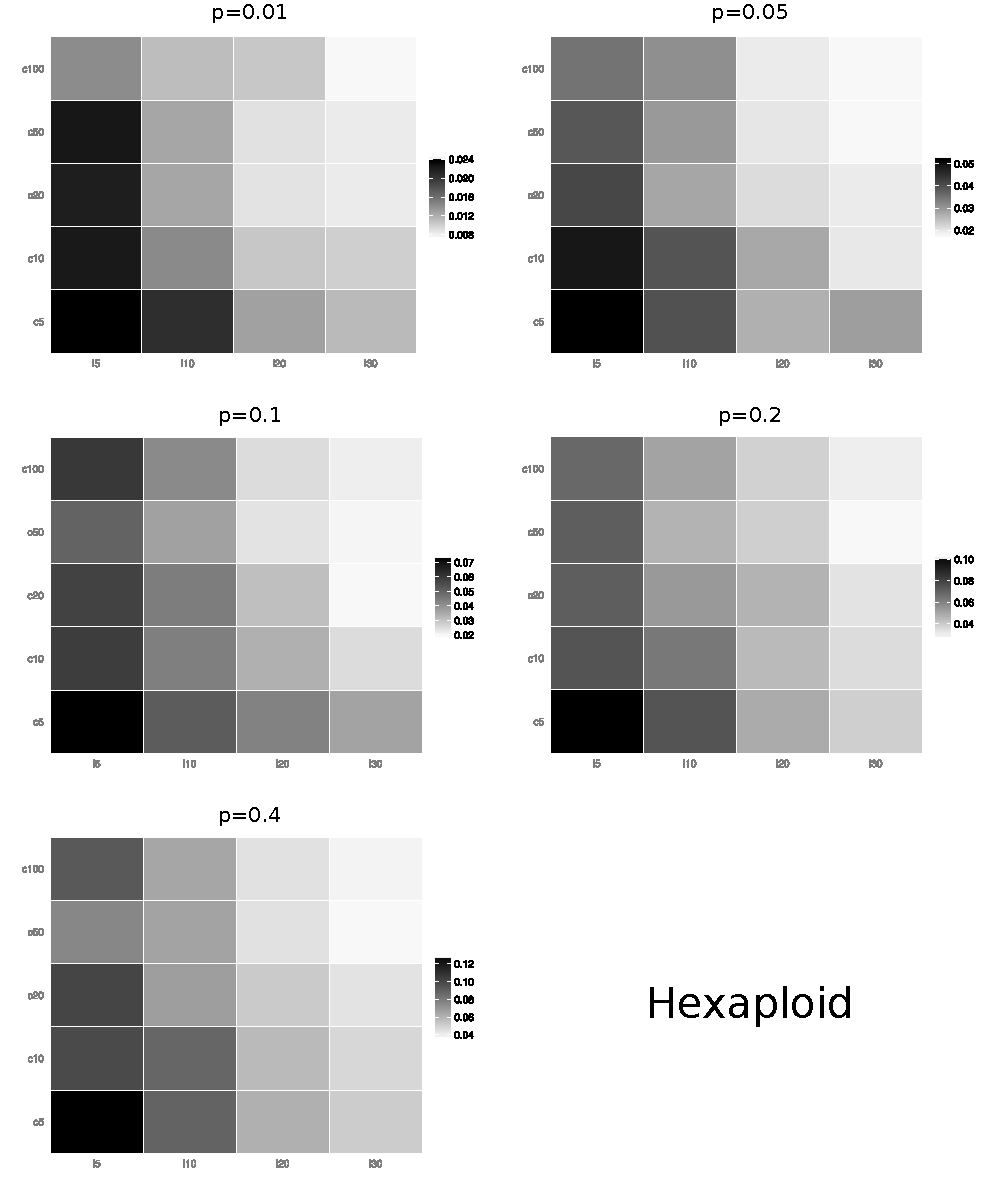
\includegraphics{fig/figure3-hex-heatmaps}
\label{fig:hex-heatmaps}
\end{figure}

\begin{figure}
\centering
\caption{\textbf{The posterior standard deviation for allele frequencies decreases with increased sequencing coverage}. This plot provides a comparison of the distribution of posterior standard deviations of the 100 replicates performed for each level of sequencing coverage for the hexaploid simulation with 30 individuals and an allele frequency of 0.2. The pointrange plots centered in the violin density plots show the mean $\pm$ 2 standard deviations.}
\vspace{0.25in}
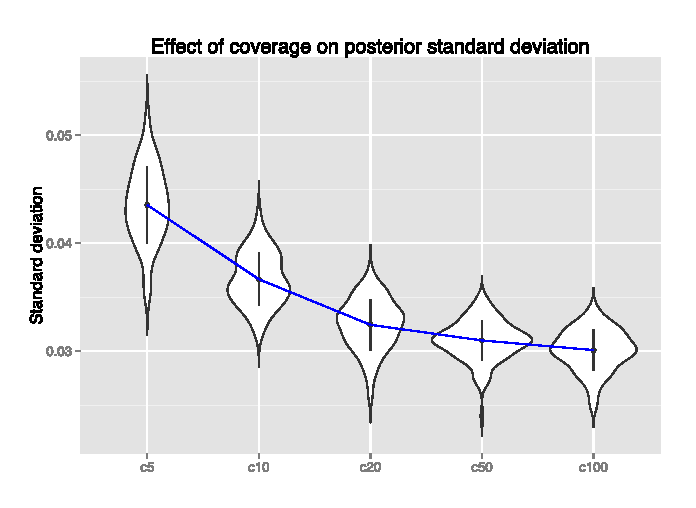
\includegraphics{fig/figure4-coverage-sd}
\label{fig:coverage-sd}
\end{figure}

\end{document}